% a-project.tex, v-1.0.3 marcoreis baseado no
% abntex2-modelo-trabalho-academico.tex, v-1.9.7 laurocesar
% Copyright 2012-2018 by abnTeX2 group at http://www.abntex.net.br/
%
% This work consists of the files ........
%
% -----------------------------------------------------------------------------
% Modelo para desenvolvimento de documentação de projetos acadêmicos
% (tese de doutorado, dissertação de mestrado e trabalhos de monografias em geral)
% em conformidade com ABNT NBR 14724:2011: Informação e documentação.
% -----------------------------------------------------------------------------
% Opções para a documentação
%
% Fancy page headings
%\documentclass[fancyheadings, subook]{Classes/a-prj}
%\documentclass[fancyheadings, sureport]{Classes/a-prj}
%
% Fancy chapters and sections headings
%\documentclass[fancychapter, subook]{Classes/a-prj}
%\documentclass[fancychapter, sureport]{Classes/a-prj}
%
% Fancy page , chapters and sections headings
%\documentclass[fancyheadings, fancychapter, subook]{Classes/a-prj}
\documentclass[fancyheadings, fancychapter, sureport]{Classes/a-report}
%
% -----------------------------------------------------------------------------
% Alguns comandos para a fancy page headings)
%
% Page header line width
%\footlinewidth{value}
%
% Page footer line width
%\headlinewidth{value}
%
% Page header and footer line width
%\headingslinewidth{value}
%
% Page header and footer lines without text
%\headingslinesonly
%
% The default line width is 0.3pt.
% Set the value to 0pt to remove the page header and/or footer line
%
% -------------------------------------------------------------------------------
% Formato de figuras suportado
% -------------------------------------------------------------------------------
% O formato das figuras depende da forma como o arquivo de saída é gerado.
% As figuras inseridas na pasta Figures serão automaticamente reconhecidas sem
% a necessidade de inserir a extensão do arquivo.
%
% O pdfLaTEX (PDF) suporta figuras com as extensões: pdf, jpg, png e mps.
%
% -------------------------------------------------------------------------------
% Árvore do diretório a-project.tex
%  Diretório
%       \Classes        (requerido)
%       \Figures        (requerido) --------------------------------->
%       \Figures\PDF    (optional)
%       \Figures\JPG    (optional) Figures located within these
%       \Figures\PNG    (optional) folders are searched automatically
%       \Figures\MPS    (optional)  by the a-prj class.
%       \Figures\EPS    (optional)
%       \Figures\PS     (optional) <--------------------------------
%       \Tables         (requerido)
%       \Others         (requerido)
%       \Chapters       (requerido)
%       \Appendices     (optional)
%       \References     (requerido)
%
% -------------------------------------------------------------------------------
% PDF File resumo
\ifpdf
    \hypersetup{
    	backref,
        colorlinks  = true,
        pdftitle    = Modelo de documentação,
        pdfauthor   = {Marco Reis, marco.a.reis@gmail.com},
        pdfsubject  = Mestre em Engenharia,
        pdfcreator  = Subtitulo,
        pdfproducer = PDFLatex,
        pdfkeywords = {documentação, latex, dissertação, tese}}
 \fi
%
% -------------------------------------------------------------------------------
% Relação de pacotes opcionais utilizados
\usepackage[utf8]{inputenc}
\usepackage[brazil]{babel}
\usepackage{longtable}
\usepackage{dcolumn}
\usepackage{multirow}
\usepackage{lscape}
%\usepackage{graphicx}
\usepackage{rotating}
%\usepackage{float,subfigure}
%\usepackage{graphicx, subfigure}
\usepackage{cite}
\usepackage[left=3cm,top=3cm,right=2cm,bottom=2cm]{geometry}
\usepackage[alf]{abntex2cite}
\usepackage{ifpdf}
\usepackage{shadow}
\usepackage{wrapfig}
\usepackage[normalem]{ulem}
\usepackage{makeidx}
\usepackage{yfonts}
\usepackage{algorithm}
\usepackage{algorithmic}
\usepackage{lmodern}
\usepackage[T1]{fontenc}
\usepackage{indentfirst}
\usepackage{color}
\usepackage{microtype}
\usepackage{lipsum}
\usepackage{caption}
\usepackage{subcaption}
\usepackage{plantuml}
\makeindex
\setlength{\LTcapwidth}{\textwidth}
%
\newtheorem{theorem}{Teorema}
\newtheorem{definition}[theorem]{Definição}
%
% -------------------------------------------------------------------------------
% Configurações do pacote backref
\renewcommand{\backrefpagesname}{Citado na(s) página(s):~}
% Texto padrão antes do número das páginas
\renewcommand{\backref}{}
% Define os textos da citação
\renewcommand*{\backrefalt}[4]{
	\ifcase #1 %
		Nenhuma citação no texto.%
	\or
		Citado na página #2.%
	\else
		Citado #1 vezes nas páginas #2.%
	\fi
}
%
% -------------------------------------------------------------------------------
% Início do documento raiz
\begin{document}
% Definição do título da página
    \university{Universidade Positivo}
	%\faculty{Programa de...}
	%\school{Escola de...}
%
    %\course{Engenharia Elétrica}
    \typework{Relatório Final}
%
	%\course{Mestrado em Modelagem Computacional e Tecnologia Industrial}
	%\typework{Disserta\c{c}\~ao de mestrado}
	%\typework{Exame de Qualificação de Mestrado}
%
	%\course{Engenharia Elétrica}
	%\typework{Tese de doutorado}
	%\typework{Exame de Qualificação de doutorado}
%
% -------------------------------------------------------------------------------
% Informações gerais
    \thesistitle{Projeto de Criação de um portfólio}
    \hidevolume
    % \thesisvolume{Volume 1 of }
    \thesisauthor{Cauê Alves};
    \thesisauthor{Vinicius Angelino};
    \thesisauthor{Pedro Karas};
    \thesisauthor{Gabriel Haiduk};
    \thesisauthor{Henrique Ribeiro};
    \thesisauthor{Equipe 10}
    \thesisadvisor{Prof. Marco Reis, M.Eng.}

    % \hidecoadvisor
    %\thesiscoadvisor{Marco Reis}
    \thesismonthyear{Junho de 2025}
%
    \maketitlepage
%
% ----------------------------------------------------------------------------
% Inserir Folha de rosto, Nota de estilo, folha de assinaturas, dedicatoria
    \begin{folharosto}
\begin{center}
\theauthor \\
\theauthorr \\
%\theauthorrr \\
%\theauthorrrr \\
%\theauthorrrrr \\
\end{center}
\ \\
\ \\
\ \\
\ \\
\ \\
\begin{spacing}{2}
   \begin{center}
   {\LARGE {\bf \thetitle}}
   \end{center}
\end{spacing}
\ \\
\ \\
\ \\
\vspace*{85mm}
% \begin{flushright}

%    \begin{list}{}{
%       \setlength{\leftmargin}{7.5cm}
%       \setlength{\rightmargin}{0cm}
%       \setlength{\labelwidth}{0pt}
%       \setlength{\labelsep}{\leftmargin}}

%       \item \thetypework apresentada ao \thefaculty, Curso de \thecourse
%       do \theuniversity, como requisito parcial para a obten\c{c}\~ao do
%       t\'itulo de {\bf \thedegreetitle}.

%       \begin{list}{}{
%       \setlength{\leftmargin}{0cm}
%       \setlength{\rightmargin}{0cm}
%       \setlength{\labelwidth}{0pt}
%       \setlength{\labelsep}{\leftmargin}}

%       \item \'Area de conhecimento: Interdisciplinar

%       \item Orientador: \theadvisor
%       \newline \hspace*{2.1cm}  %{\it \theuniversity}

%       \end{list}
%    \end{list}

% \end{flushright}
\ \\
\ \\
\ \\
\ \\
%\begin{spacing}{1.5}
   \begin{center}
   Curitiba \par
   \theuniversity \par
   2025
   \end{center}
%\end{spacing}

\end{folharosto}

    %\begin{notaestilo}
Esta \thetypeworkthree foi elaborada considerando as normas de
estilo (i.e. est\'eticas e estruturais) propostas aprovadas pelo
colegiado do \thefacultytwo e est\~ao dispon\'iveis em formato
eletr\^onico ({\it download} na P\'agina Web
http:$//$ead.fieb.org.br$/$portal\_faculdades$/$dissertacoes-e-teses-mcti.html
ou solicita\c{c}\~ao via e-mail \`a secretaria do
programa) e em formato impresso somente para consulta. \\

Ressalta-se que o formato proposto considera diversos itens das
normas da Associa\c{c}\~ao Brasileira de Normas T\'ecnicas (ABNT),
entretanto opta-se, em alguns aspectos, seguir um estilo pr\'oprio
elaborado e amadurecido pelos professores do programa de
p\'os-gradua\c{c}\~ao supracitado.

\end{notaestilo}

    %\include{Others/FolhaAssinaturas}
    %\include{Others/dedicatoria}
    %\include{Others/agradecimentos}
%
% ----------------------------------------------------------------------------
% Resumo/abstract, sumário e siglas
    \begin{romanpagenumbers}
        \begin{thesisresumo}
O projeto que apresentamos hoje se concentra na criação de um portfólio profissional para um cliente. Adicionamos todas as informações solicitadas na primeira reunião que tivemos com ele. Analisamos todos os seus desejos e os colocamos em ordem para a execução final. O projeto em si visa destacar todas as habilidades, experiências e gostos do cliente, atraindo a atenção de empresas e recrutadores para uma possível contratação.
\ \\

% use de três a cinco palavras-chave

\textbf{Palavras-chave}: Portfólio, Profissional, Perfil pessoal, Cliente, Projetos

\end{thesisresumo}

        \begin{thesisabastract}
The project we are presenting today focuses on creating a professional portfolio for a client. We added all the information requested in the first meeting we had with him. We took all his wishes and put them in order for final execution. The project itself aims to showcase all the client's skills, experiences and tastes, making him attract the attention of companies and recruiters for a possible hiring.
\ \\

\textbf{Keywords}: Portfolio, Professional, Personal profile, Customer, Project

\end{thesisresumo}

        % Make list of contents, tables and figures
        \thesiscontents
        % \pdfbookmark[1]{Lista de Tabelas}{lot} \listoftables
        \newpage
        %Include other required section
        %\begin{thesisabbreviations}
\begin{footnotesize}
\begin{longtable}[l]{p{2cm}l}
  tprax   \dotfill & \thefaculty \\
  WWW       \dotfill &  World Wide Web \\
\end{longtable}
\end{footnotesize}
\end{thesisabbreviations}

        %\begin{thesissymbols}
\begin{footnotesize}
\begin{longtable}[l]{p{2cm}l}
  $\partial$   \dotfill  & Bla bla bla \\
  $\prod$       \dotfill & ble ble ble \\
  $\partial$   \dotfill  & Bla bla bla \\
  $\prod$       \dotfill & ble ble ble \\
  $\partial$   \dotfill  & Bla bla bla \\
  $\prod$       \dotfill & ble ble ble \\
  $\partial$   \dotfill  & Bla bla bla \\
  $\prod$       \dotfill & ble ble ble \\
  $\partial$   \dotfill  & Bla bla bla \\
  $\prod$       \dotfill & ble ble ble \\
  $\partial$   \dotfill  & Bla bla bla \\
  $\prod$       \dotfill & ble ble ble \\
  $\partial$   \dotfill  & Bla bla bla \\
  $\prod$       \dotfill & ble ble ble \\
  $\partial$   \dotfill  & Bla bla bla \\
  $\prod$       \dotfill & ble ble ble \\
  $\partial$   \dotfill  & Bla bla bla \\
  $\prod$       \dotfill & ble ble ble \\
  $\partial$   \dotfill  & Bla bla bla \\
  $\prod$       \dotfill & ble ble ble \\
  $\partial$   \dotfill  & Bla bla bla \\
  $\prod$       \dotfill & ble ble ble \\
  $\partial$   \dotfill  & Bla bla bla \\
  $\prod$       \dotfill & ble ble ble \\
  $\partial$   \dotfill  & Bla bla bla \\
  $\prod$       \dotfill & ble ble ble \\
  $\partial$   \dotfill  & Bla bla bla \\
  $\prod$       \dotfill & ble ble ble \\
  $\partial$   \dotfill  & Bla bla bla \\
  $\prod$       \dotfill & ble ble ble \\
  $\partial$   \dotfill  & Bla bla bla \\
  $\prod$       \dotfill & ble ble ble \\
  $\partial$   \dotfill  & Bla bla bla \\
  $\prod$       \dotfill & ble ble ble \\
  $\partial$   \dotfill  & Bla bla bla \\
  $\prod$       \dotfill & ble ble ble \\
  $\partial$   \dotfill  & Bla bla bla \\
  $\prod$       \dotfill & ble ble ble \\          
\end{longtable}
\end{footnotesize}
\end{thesissymbols}

        %Switch the page numbering back to the default format
    \end{romanpagenumbers}
%
% ---------------------------------------------------------------------------
% Include thesis chapters
    \parskip=\baselineskip
    \chapter{Introdução}
\label{chap:intro}
Este projeto consiste em desenvolver um portifólio profissional para nosso cliente, tendo em meta a utilização para por em seus curriculos e projetos. 

\section{Objetivos}
\label{sec:obj}
O projeto tem como objetivos, o desenvolvimento do portfólio do cliente, atrair novas oportunidades, desenvolver um profissional capacitado, aprimorar ou
desenvolver habilidades e competencias e o aprendizado.

\subsection{Objetivos Específicos}
\label{ssec:objesp}
Os objetivos específicos deste projeto são:
\begin{itemize}
      \item Desenvolver portifólio ao cliente.
      \item Demonstrar habilidades e competencias;
      \item Transmitir profissionalismo;
      \item Atrair novas oportunidades;
  \end{itemize}

% \subsubsection*{Objetivos específicos principais}
% \label{sssec:obj-principais}

%--------- NEW SECTION ----------------------
\section{Justificativa}
\label{sec:justi}

O desenvolvedor deverá realizar a programação de um portifólio profissional para o cliente, contendo todas as informações pedidas nele.




%--------- NEW SECTION ----------------------
\section{Organização do documento}
\label{section:organizacao}

Este documento apresenta $5$ capítulos e está estruturado da seguinte forma:

\begin{itemize}

  \item \textbf{Capítulo \ref{chap:intro} - Introdução}: Contextualiza o âmbito, no qual o projeto foi desenvolvido. Apresenta, portanto, a definição do problema, objetivos e justificativas do projeto e como este \thetypeworkthree está estruturado;
  \item \textbf{Capítulo \ref{chap:fundteor} - Fundamentação Teórica}: Contextualiza o inicio do projeto. A busca por informações para iniciar e deselvolver o portfolio.;
  \item \textbf{Capítulo \ref{chap:metod} - Materiais e Métodos}: Nos mostra, materiais e metodologias que foram usadas no desenvolvimento do projeto;
  \item \textbf{Capítulo \ref{chap:result} - Resultados}: Apresenta os resultaos que foram gerados por meio do projeto ao longo de seu desenvolvimento;
  \item \textbf{Capítulo \ref{chap:conc} - Conclusão}: Apresenta as conclusóes, contribuições e algumas sugestões de atividades de pesquisa a serem desenvolvidas no futuro.

\end{itemize}

    \chapter{Conceito do projeto do portfólio}
\label{chap:fundteor}
%--------- NEW SECTION ----------------------
O portifólio tem como objetivo de demonstrar todo o interesse do cliente para empresas visitarem e talvez chamarem para entrevistas.
% isso é igual <=  === <> #{ #( www
% <| |>
% ===

Lista dos documentos
\begin{enumerate}
   \item diagrama de classe
   \item diagrama de casos de uso
   \item diagrama de sequência
\end{enumerate}

O desenvolvimento do projeto consiste na criação de um projeto para o nosso cliente que pediu um portifólio demonstrando toda carreira profissinal dele até hoje, assim recurtadores poderão entrar em contato com ele via portifólio.

Neste capítulo serão abordados os requisitos do cliente e os requisitos funcionais.



%conferir se precisa de requisitos do cliente
\section{Requisitos do cliente}
 O cliente definiu certos requisitos quanto à operação e às características do potifólio:
 \begin{itemize}
    \item Informações pessoais (nome, cidade e idade);
    \item Curta descrição sobre conhecimentos de manutenção de computadores e que mexe com computadores desde os 3 anos de idade.;
    \item Cores a serem utilizadas: preto, branco e cinza;
    \item Inserir experiencia de trabalho (2x suporte);
    \item Listar as acadêmicas (conhecimentos);
    \item Colocar as áreas de interesse;
    \item Hobbies;
    \item Não utilizar foto pessoal;
    \item Colocar o GitHub;
    \item Adicionar informações dos projetos desenvolvidos;
    \item portfolio minimalista;
 \end{itemize}

\section{Requisitos funcionais}
 Com base nos requisistos dados pelo cliente, foi realizado uma análise e filtragem, e assim selecionados somente os requisistos que são funcionais.
 \begin{itemize}
    \item Exibir informações pessoais: nome, cidade e idade;
    \item Mostrar uma curta descrição sobre conhecimentos em manutenção de computadores e que mexe com computadores desde os 3 anos;
    \item Inserir experiência de trabalho (duas vezes como suporte);
    \item Listar formação ou conhecimentos acadêmicos;
    \item Informar as áreas de interesse;
    \item Exibir os hobbies;
    \item Colocar o GitHub;
    \item Adicionar informações dos projetos desenvolvidos;
 \end{itemize}




 


 

 
 

 


    \chapter{Desenvolvimento do projeto}
\label{chap:metod}
Nesta seção será descrito o procedimento utilizado para construção inicial do portifólio pedido pelo cliente.
\section{Metodologia do projeto}
A metodologia utilizada para o desenvolvimento deste projeto foi baseada no modelo \textit{kanban}, que é um modelo de desenvolvimento que visa otimizar o fluxo de trabalho e a entrega de valor. Este modelo é caracterizado por um sitema visual, onde tarefas são representadas por cartões que se movem ao longo de colunas, representando o andamento do projeto. As colunas que representam as fases do modelo \textit{kanban} incluem: a fazer, em progresso, checagem, e concluido.

\section{Ideação}
  Depois da primeira reunião com o cliente e da retirada dos requisitos, já conseguimos identificar que nosso cliente é do tipo mais simples, e com base nisso decidimos criar um site/portfólio que fosse simples e prático, com isso em mente tivemos a ideia de criar um site one page com todas as informações principais do nosso cliente.

\section{Arquitetura Geral}
 A arquitetura geral, apresentada na Figura \ref{fig:arquitetura_geral}, relaciona de modo geral a interface do usuário, com a central de gerenciamento do site. Neste contexto, a interface do usuário representa o contato direto com o usuário por meio de site.
Para a central de gerenciamento do site utilizou-se o VScode. Neste cojunto se encontram as principais funcionalidades do site: mostrar as informações do cliente, navegação, atrair empregadores e empregar o cliente. Por fim, no conjunto de saídas estão os elemetos visuais.
\begin{figure} [h!]	
    \centering
    \caption{Minha arquitetura geral}
    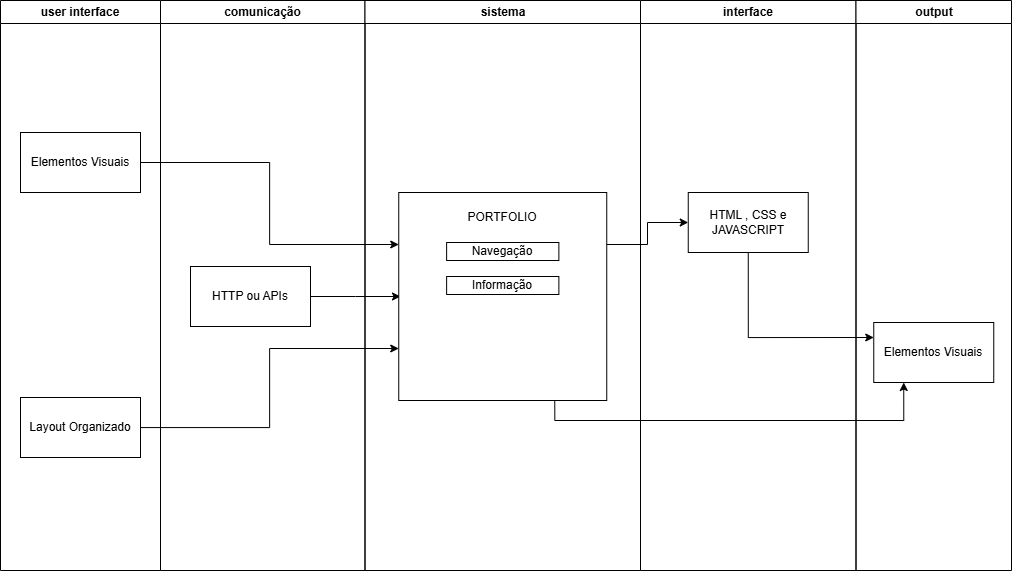
\includegraphics[width=0.8\textwidth]{Figures/arquitetura-solução.png}
    \caption*{Fonte: Autoria própria.}
    \label{fig:arquitetura_geral}
\end{figure}

\section{Requisitos técnicos}
 O portfólio foi desenvolvido em HTML e CSS, porem não contém mais requisitos tecnicos, foi um desenvolvimento mas básico.

\section{Modelagem dos processos}
 Modelagem dos processos \ref{fig:modelagem_processos} é uma técnica utilizada para representar, analisar, melhorar e automatizar os processos de uma organização. Ela descreve como as atividades são realizadas, quem as executa, quais recursos são usados e quais resultados são produzidos.
 \begin{figure} [h!]	
    \centering
    \caption{Minha modelagem de processos}
    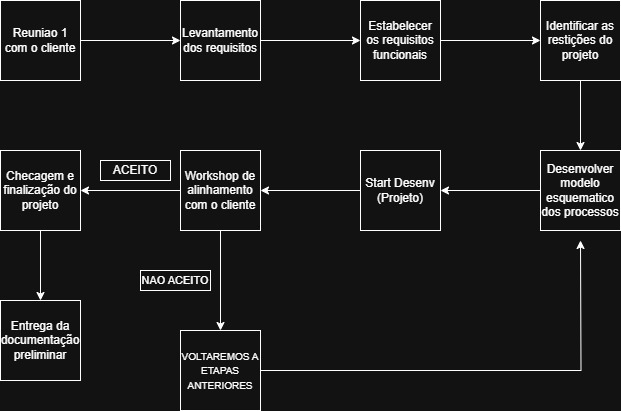
\includegraphics[width=0.8\textwidth]{Figures/modelagem_processos.jpeg}
    \caption*{Fonte: Autoria própria.}
    \label{fig:modelagem_processos}
\end{figure}
    \chapter{Resultados}
\label{chap:result}
Aqui trataremos sobre os resultados que foram encontrados durante o desenvolvimentodo projeto. Foi um projeto extenso e com dificuldades em certos momentos, porém, no fim conseguimos conclui-lo e trazer os resultados deste projeto à tona.


\section{Diagrama de classes}
\label{sec:class}
O diagrama de classes é uma representação visual das classes do sistema e seus relacionamentos. 
\begin{figure} [h!]	
    \centering
    \caption{Meu diagrama de classes}
    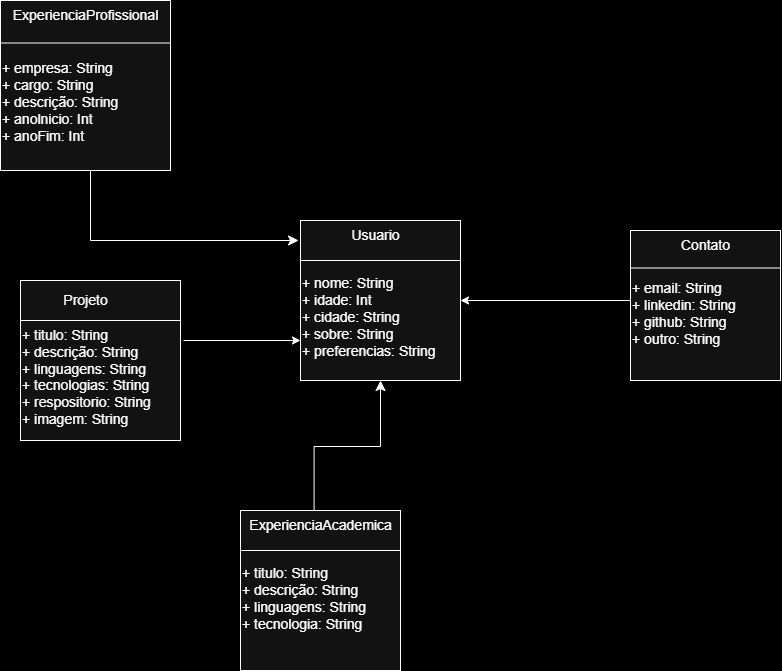
\includegraphics[width=0.8\textwidth]{Figures/diagrama-de-classes.png}
    \caption*{Fonte: Autoria própria.}
    \label{fig:diagrama_classes}
\end{figure}

favor olhar a seção \ref{sec:class}.


\section{Diagrama de casos de uso}
\label{sec:casos}
O diagrama de casos de uso é uma representação visual dos casos de uso do sistema e os atores envolvidos. Ele é utilizado para descrever as funcionalidades do sistema e como os usuários interagem com ele. A Figura \ref{fig:diagrama_casos} apresenta o diagrama de casos de uso do projeto desenvolvido.
\begin{figure} [h!]	
    \centering
    \caption{Meu diagrama de casos de uso}
    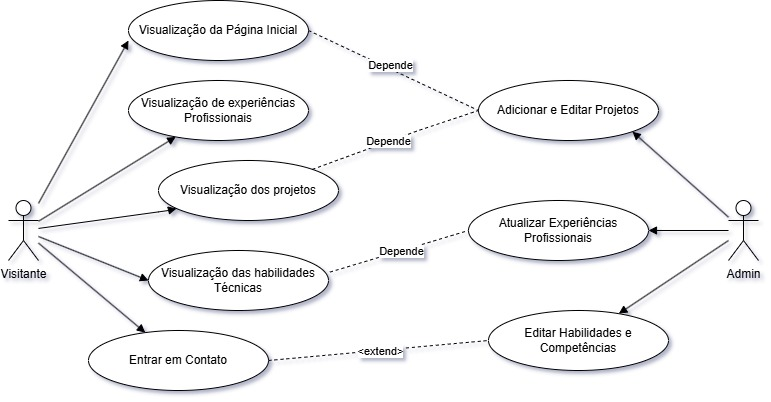
\includegraphics[width=0.8\textwidth]{Figures/diagrama-casos-de-uso.jpeg}
    \caption*{Fonte: Autoria própria.}
    \label{fig:diagrama_casos}
\end{figure}


\section{Diagrama de sequência}
\label{sec:sequencia}   
O diagrama de sequência é uma representação visual da interação entre os objetos do sistema ao longo do tempo. Ele é utilizado para descrever como os objetos interagem entre si para realizar uma determinada funcionalidade. A Figura \ref{fig:diagrama_sequencia} apresenta o diagrama de sequência do projeto desenvolvido. 
\begin{figure} [h!]	
    \centering
    \caption{Meu diagrama de sequencia}
    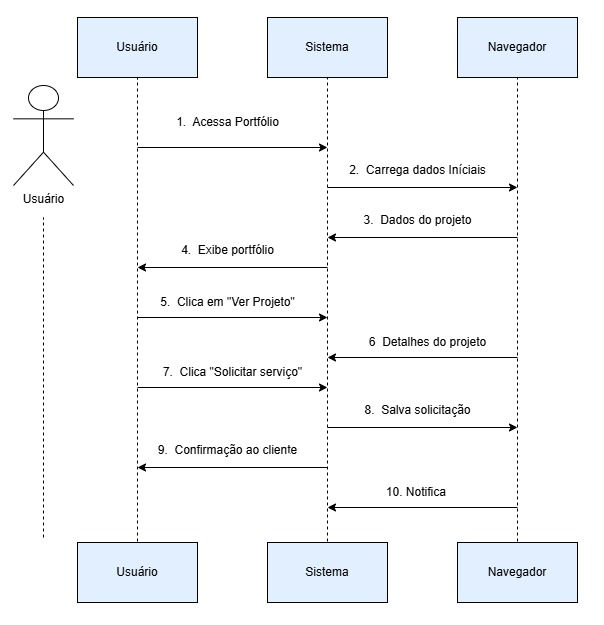
\includegraphics[width=0.8\textwidth]{Figures/diagrama-de-sequencia.jpeg}
    \caption*{Fonte: Autoria própria.}
    \label{fig:diagrama_sequencia}
\end{figure}








    \chapter{Conclusão}
\label{chap:conc}

Chegou a hora de apresentar o apanhado geral sobre o desenvolvimento do
projeto feito, no qual s\~ao sintetizadas uma s\'erie de
reflex\~oes sobre a metodologia usada, sobre os achados e
resultados obtidos. A partir da construção deste projeto, foi idealizado
uma base de como seria o portfolio do nosso cliente, e ao final do projeto,
acreditamos que conseguimos alcançar aquela ideia inicial e até melhorar ela.


\section{Considerações finais}
\label{sec:consid}

Considerando tudo o que foi dito e mostrado, é muito interresante dizer
que este projeto foi um marco muito legal para um primeiro desenvolvimento. 
Foi complicado e desafiador, porém, estimulante e com um grande carga de 
aprendizado.


    % include more chapters ...
%
% ----------------------------------------------------------------------------
% Include thesis appendices
    \begin{thesisappendices}
        % Thesis Appendix -------------------------------------------------------

% \chapter{Diagramas mecânicos}
% \label{Append:diagmec}



        % Thesis Appendix -------------------------------------------------------

% \chapter{Diagramas eletro-eletrônicos}
% \label{Append:diagele}



        %% Thesis Appendix -------------------------------------------------------

\chapter{Logbook}
\label{Append:log}



    \end{thesisappendices}
%
% ----------------------------------------------------------------------------
% Configurar as referencias bibliograficas
	% \renewcommand\bibname{Referências}
    % \addcontentsline{toc}{chapter}{Referências}
    % \bibliography{References/referencias}
%
% ----------------------------------------------------------------------------
% Finishing him
    \include{Others/ultimafolha}
\end{document}
%
% -------------------------------------------------------------------------------
% Aqui termina a formatação para o documento.
% In God We Trust. All Other Bring Data.
%
% -------------------------------------------------------------------------------